\section{Deep-Unfolded Receiver Design}
\label{sec:algorithm}

From the posterior factorization in \eqref{eq:working-posterior}, we
derive Gaussian messages linking linear estimation to channel and
activity denoising, then parameterize the denoisers and message
variances to obtain $L$ trainable layers.

\subsection{Factor Graph Representation}

Let $J=KN$ and $C=MN$, and denote column $c$ of $\mathbf X$ and
$\mathbf Y$ by $\mathbf x_c$ and $\mathbf y_c$, respectively.
The observation factor is
\begin{equation}
 f_{\rm y}(\mathbf X)
 =\prod_{c=1}^{C}\CN(\mathbf y_c;
       \mathbf A_{\rm c}\mathbf x_c,\sigma_{\rm c}^2\I_Q),
 \label{eq:twc-factor-definitions}
\end{equation}
while each user's factors comprise the activity prior
$f_{\alpha,k}(\alpha_k)=\rho^{\alpha_k}(1-\rho)^{1-\alpha_k}$,
the channel prior $q_{\rm tr}(dH_k)$, and the constraint $g_k$
enforcing $X_k=\alpha_kH_k$. Figure~\ref{fig:twc-factor-graph}
shows their connections, with each $H_k$ node retaining the joint
distribution of the complete channel tensor.

\begin{figure}[t]
\centering
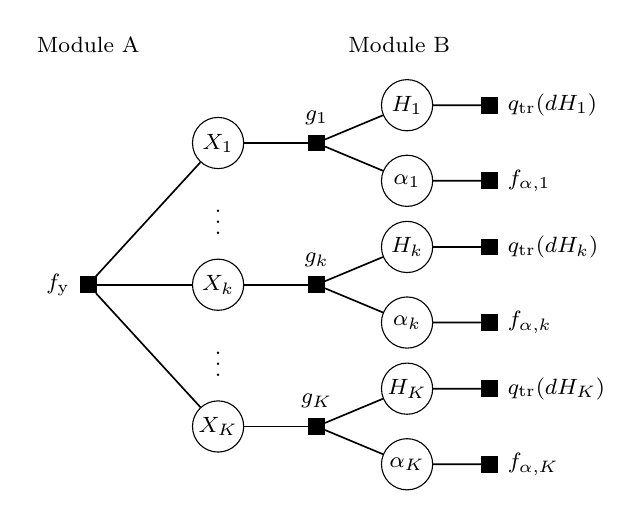
\begin{tikzpicture}[
 font=\footnotesize,
 fgvariable/.style={circle,draw,minimum size=6.5mm,inner sep=1pt},
 fgfactor/.style={rectangle,draw,fill=black,minimum size=2mm,inner sep=0pt},
 fgedge/.style={semithick}]
 \node[fgfactor,label=left:{$f_{\rm y}$}] (fy) at (0,0) {};
 \node[align=center] at (0,3.05) {Module A};
 \node[align=center] at (3.95,3.05) {Module B};
 \foreach \idx/\row in {1/1.8,k/0,K/-1.8} {
   \node[fgvariable] (x\idx) at (1.65,\row) {$X_{\idx}$};
   \node[fgfactor,label=above:{$g_{\idx}$}] (g\idx) at (2.9,\row) {};
   \node[fgvariable] (h\idx) at (4.05,{\row+0.48}) {$H_{\idx}$};
   \node[fgvariable] (a\idx) at (4.05,{\row-0.48}) {$\alpha_{\idx}$};
   \node[fgfactor,label=right:{$q_{\rm tr}(dH_{\idx})$}]
       (ph\idx) at (5.1,{\row+0.48}) {};
   \node[fgfactor,label=right:{$f_{\alpha,\idx}$}]
       (pa\idx) at (5.1,{\row-0.48}) {};
   \draw[fgedge] (fy) -- (x\idx);
   \draw[fgedge] (x\idx) -- (g\idx);
   \draw[fgedge] (g\idx) -- (h\idx) -- (ph\idx);
   \draw[fgedge] (g\idx) -- (a\idx) -- (pa\idx);
 }
 \node at (1.65,0.9) {$\vdots$};
 \node at (1.65,-0.9) {$\vdots$};
\end{tikzpicture}
\caption{Factor graph of \eqref{eq:working-posterior}, with the
observation factors grouped into $f_{\rm y}$. Circles denote variable
nodes and filled squares denote factor nodes. Each $X_k$ or $H_k$
node contains $D$ complex coefficients. The likelihood couples the
user blocks, while $g_k$ imposes $X_k=\alpha_kH_k$.}
\label{fig:twc-factor-graph}
\end{figure}


Following \cite{cai2026}, module A groups $f_{\rm y}$ for column-wise
linear estimation, while module B groups the user constraints and
priors for channel and activity denoising. Conditioned on the messages
from A, the factors in B separate over users, whose blocks are obtained
by \eqref{eq:mmv-indexing}. The modules exchange Gaussian extrinsic
messages \cite{minka2001,cai2026}, denoted by
$\mathcal M_{\rm A\to B}^{(\ell)}$ and
$\mathcal M_{\rm B\to A}^{(\ell)}$ at layer $\ell$. Each module
combines its factors with the incoming message to form a local belief,
then divides its Gaussian approximation by that message to remove
the incoming contribution, following the flow in
Fig.~\ref{fig:twc-receiver}.

\begin{figure*}[t]
\centering
\begin{tikzpicture}[
 font=\footnotesize,
 block/.style={draw,rounded corners=1pt,align=center,
               minimum height=0.85cm,inner sep=5pt},
 flow/.style={-{Latex[length=2mm]},semithick},
 supervision/.style={-{Latex[length=1.7mm]},dashed},
 loss/.style={draw,dashed,align=center,inner sep=4pt}]
 \node[block,text width=2.1cm] (front) at (1.2,2.7)
 {Phase and noise\\estimation; normalization};
 \node[above=3mm of front] (obs) {$\mathbf Y,P,\rho$};
 \node[block,text width=2.0cm] (init) at (4.25,2.7)
 {Initialize\\$\mathbf M_1=0$\\$w_1=\rho P_H$};
 \node[block,text width=2.25cm] (linear) at (4.25,0.75)
 {Linear estimation\\and extrinsic message\\\eqref{eq:twc-linear-correction}--\eqref{eq:twc-query-calibrated}};
 \node[block,text width=2.2cm] (score) at (7.75,1.8)
 {Channel denoising\\$\mu_{k\ell}$ from \eqref{eq:twc-conditional-mean}};
 \node[block,text width=2.25cm] (activity) at (10.65,0)
 {Activity classifier\\$p_{k\ell}$ from \eqref{eq:twc-activity}};
 \node[block,text width=1.5cm] (product) at (13.8,1.8)
 {$\widehat x_{k\ell}$\\$=p_{k\ell}\mu_{k\ell}$};
 \node[block,text width=3.1cm] (feedback) at (13.8,-2.15)
 {Residual, variance, and\\extrinsic message with damping\\\eqref{eq:twc-residual-scale}--\eqref{eq:twc-damping}};
 \node[loss] (lossH) at (7.75,3.5)
 {Active-channel loss $R_H^{(\ell)}$};
 \node[loss] (lossA) at (10.65,-1.15)
 {Activity loss $R_a^{(\ell)}$};
 \draw[flow] (obs) -- (front);
 \draw[flow] (front.south) |- node[pos=0.72,above]
 {$\mathbf Y,\mathbf A_{\rm c},\sigma_{\rm c}^2$} (linear.west);
 \draw[flow] (init) -- (linear);
 \coordinate (split) at (5.9,0.75);
 \draw[flow] (linear.east) -- (split) |- (score.west);
 \draw[flow] (split) |- node[pos=0.73,below] {$u_{k\ell},v_\ell,\rho$}
 (activity.west);
 \node[above] at (5.95,1.8) {$u_{k\ell},v_\ell$};
 \draw[flow] (score.east) -- node[above] {$\mu_{k\ell}$} (product.west);
 \draw[flow] (10.65,1.8) -- (activity.north);
 \draw[flow] (activity.east) -| node[pos=0.3,below] {$p_{k\ell}$}
 (product.south);
 \draw[flow] (product.east) -- (16.5,1.8)
 node[above,align=center] {Output\\at $\ell=L$};
 \draw[flow] (16.1,1.8) |- (feedback.east);
 \node[right,align=left] at (16.15,-0.8) {$\ell<L$};
 \draw[flow] (feedback.west) -- (4.25,-2.15) -- (linear.south);
 \node[above] at (7.65,-2.15) {$\mathbf M_{\ell+1},w_{\ell+1}$};
 \node[below,align=center] at (13.8,-2.9)
 {uses $\mathbf Y,\mathbf A_{\rm c},\sigma_{\rm c}^2$};
 \draw[supervision] (score) -- (lossH);
 \draw[supervision] (activity) -- (lossA);
\end{tikzpicture}
\caption{Receiver message flow. User estimates are assembled before
the residual is computed; feedback also uses the current messages
$\mathbf R_\ell,v_\ell,\mathbf M_\ell,w_\ell$.
Dashed connections denote training losses, whose gradients propagate
through the networks and inter-layer messages.}
\label{fig:twc-receiver}
\end{figure*}

\subsection{Linear Estimation}

At layer $\ell$, the input Gaussian messages have means collected in
$\mathbf M_\ell$ and a common covariance $w_\ell\I_J$ for each
column of $\mathbf X$. Let $\mathbf m_{\ell c}$ be column $c$ of
$\mathbf M_\ell$. The input message and the belief at $f_{\rm y}$
are
\begin{equation}
 \begin{aligned}
 \mathcal M_{\rm B\to A}^{(\ell)}(\mathbf X)
 &=\prod_{c=1}^{C}\CN(\mathbf x_c;
                  \mathbf m_{\ell c},w_\ell\I_J),\\
 b_{\rm A}^{(\ell)}(\mathbf X)
 &\propto f_{\rm y}(\mathbf X)
             \mathcal M_{\rm B\to A}^{(\ell)}(\mathbf X).
 \end{aligned}
 \label{eq:twc-linear-belief}
\end{equation}
Completing the square in \eqref{eq:twc-linear-belief} gives the mean
$\mathbf M_\ell+\bm\Delta_\ell$ and average marginal variance
$t_\ell$, where
\begin{equation}
 \begin{aligned}
 \bm\Delta_\ell&=w_\ell\mathbf A_{\rm c}^{\mathsf H}
 (\sigma_{\rm c}^2\I_Q+w_\ell\mathbf A_{\rm c}\mathbf A_{\rm c}^{\mathsf H})^{-1}
 (\mathbf Y-\mathbf A_{\rm c}\mathbf M_\ell),
 \\
 t_\ell&=\frac1J\tr\!\left[
 \left(w_\ell^{-1}\I_J+
 \frac{\mathbf A_{\rm c}^{\mathsf H}\mathbf A_{\rm c}}{\sigma_{\rm c}^2}
 \right)^{-1}\right].
 \end{aligned}
 \label{eq:twc-linear-correction}
\end{equation}
Matching these moments gives a Gaussian approximation
$\widehat b_{\rm A}^{(\ell)}$ with covariance $t_\ell\I_J$ per
column, whose quotient with $\mathcal M_{\rm B\to A}^{(\ell)}$
gives the extrinsic variance and mean \cite{minka2001,cai2026}:
\begin{equation}
 \begin{aligned}
 v_\ell^{(0)}&=(t_\ell^{-1}-w_\ell^{-1})^{-1},\\
 \mathbf R_\ell^{(0)}&=v_\ell^{(0)}
 \left(\frac{\mathbf M_\ell+\bm\Delta_\ell}{t_\ell}
       -\frac{\mathbf M_\ell}{w_\ell}\right).
 \end{aligned}
 \label{eq:twc-linear-extrinsic}
\end{equation}
Because the Gaussian quotient links the mean and variance, we adjust
both when introducing the trainable scale
$\gamma_\ell=e^{c_{\gamma,\ell}}>0$. With
$v_\ell=\gamma_\ell v_\ell^{(0)}$, requiring the product of the
incoming and outgoing messages to retain mean
$\mathbf M_\ell+\bm\Delta_\ell$ gives
$(v_\ell\mathbf M_\ell+w_\ell\mathbf R_\ell)/(w_\ell+v_\ell)
=\mathbf M_\ell+\bm\Delta_\ell$, and hence
\begin{equation}
 v_\ell=\gamma_\ell v_\ell^{(0)},\qquad
 \mathbf R_\ell=\mathbf M_\ell+
 \left(1+\frac{v_\ell}{w_\ell}\right)\bm\Delta_\ell.
 \label{eq:twc-query-calibrated}
\end{equation}
The pair $(\mathbf R_\ell,v_\ell)$ is passed to module B, reducing
to \eqref{eq:twc-linear-extrinsic} when $\gamma_\ell=1$.

\subsection{Channel and Activity Denoising}

Rearrange $\mathbf R_\ell$ into user blocks according to
\eqref{eq:mmv-indexing}, and let $r_{k\ell}\in\mathbb C^D$ be the
vectorized block for user $k$. The Gaussian message passed to module B
is
\begin{equation}
 \mathcal M_{\rm A\to B}^{(\ell)}(\mathbf X)
 =\prod_{k=1}^{K}\CN\!\left(\vect(X_k);
                       r_{k\ell},v_\ell\I_D\right).
 \label{eq:twc-denoiser-message}
\end{equation}
At $g_k$, the constraint $X_k=\alpha_kH_k$ gives the likelihood
$\CN(r;\alpha h,v\I_D)$, where we omit the user and layer indices
and write $h=\vect(H_k)$ and $r=r_{k\ell}$. Integrating over the
channel under each activity hypothesis gives
\begin{equation}
 \begin{aligned}
 q_0(r;v)&=\CN(r;0,v\I_D),\\
 q_1(r;v)&=\int\CN(r;h,v\I_D)\,q_{\rm tr}(dh).
 \end{aligned}
 \label{eq:twc-local-densities}
\end{equation}
Multiplying by the activity prior $f_{\alpha,k}$ and normalizing
gives the joint channel and activity belief
\begin{equation}
 \begin{gathered}
 q(dh,a\mid r,v)=
 \frac{\rho^a(1-\rho)^{1-a}\CN(r;ah,v\I_D)\,q_{\rm tr}(dh)}
 {(1-\rho)q_0(r;v)+\rho q_1(r;v)},\\
 a\in\{0,1\}.
 \end{gathered}
 \label{eq:twc-local-posterior}
\end{equation}
Conditioning \eqref{eq:twc-local-posterior} on the active hypothesis
gives the conditional channel mean
\begin{equation}
 \mu^\star(r,v)=\E[h\mid r,\alpha=1]
 =\frac{\int h\,\CN(r;h,v\I_D)\,q_{\rm tr}(dh)}{q_1(r;v)}.
 \label{eq:twc-local-channel-target}
\end{equation}
The activity probability follows from Bayes' rule as
\begin{equation}
 p^\star(r,v)=\Pr(\alpha=1\mid r)
 =\frac{\rho q_1(r;v)}
 {(1-\rho)q_0(r;v)+\rho q_1(r;v)}.
 \label{eq:twc-local-activity-target}
\end{equation}
Since $x=\alpha h$ vanishes under the inactive hypothesis, averaging
over the two activity states gives \cite{cai2026}
\begin{equation}
 \E[x\mid r]=p^\star(r,v)\mu^\star(r,v).
 \label{eq:twc-mixture-mean}
\end{equation}
Evaluating $\mu^\star$ and $p^\star$ requires integration over the
$D$-dimensional channel distribution for every user and layer, so we
approximate them with a score-based denoiser and an activity classifier.

Let $u_{k\ell}\in\mathbb R^{2D}$ denote the real and imaginary parts
of the denoiser input for user $k$. Based on the score representation developed
in Section~\ref{sec:learning}, the channel estimate is
\begin{equation}
 \mu_{k\ell}=u_{k\ell}
       +a_\ell\frac{v_\ell}{2}s_{\theta_\ell}(u_{k\ell},v_\ell),
 \qquad a_\ell=e^{c_{\alpha,\ell}}.
 \label{eq:twc-conditional-mean}
\end{equation}
Here $s_{\theta_\ell}$ is the score network in layer $\ell$,
$v_\ell/2$ is the noise variance per real coordinate, and $a_\ell$
controls the denoising correction.

For the classifier, rewriting \eqref{eq:twc-local-activity-target}
in terms of posterior odds gives
\begin{equation}
 \logit p^\star(r,v)
 =\logit(\rho)+\log\frac{q_1(r;v)}{q_0(r;v)}.
 \label{eq:twc-activity-odds}
\end{equation}
Representing the likelihood-ratio term by a trainable log-odds
correction \cite{menon2016}, the classifier uses the input and
conditional channel estimate to compute
\begin{equation}
 p_{k\ell}=\sigmoid\!\left(\logit(\rho)+
 g_{\phi_\ell}(u_{k\ell},v_\ell,\mu_{k\ell},\rho)\right),
 \label{eq:twc-activity}
\end{equation}
where $\phi_\ell$ denotes the classifier parameters.
Substituting the channel and activity estimates into
\eqref{eq:twc-mixture-mean} gives
\begin{equation}
 \widehat x_{k\ell}=p_{k\ell}\mu_{k\ell}.
 \label{eq:twc-estimate}
\end{equation}
The estimates form $\widehat{\mathbf X}_\ell$ after conversion to
complex form and rearrangement by \eqref{eq:mmv-indexing}.
All users share the networks within a layer, with soft probabilities
retained until the final activity decision.

\subsection{Extrinsic Message Update}

To form the Gaussian return message, we associate
$\widehat{\mathbf X}_\ell$ with a common scalar variance, which we
estimate from the observation residual. Under the fixed-parameter
model, a zero-mean error with covariance $\tau\I_J$
per column and uncorrelated with the noise would satisfy
\[
 \E\|\mathbf Y-\mathbf A_{\rm c}\widehat{\mathbf X}_\ell\|_F^2
 =C\tau\|\mathbf A_{\rm c}\|_F^2+QC\sigma_{\rm c}^2.
\]
This relation motivates the normalized residual quantity
\begin{equation}
 e_\ell=\frac{\|\mathbf Y-\mathbf A_{\rm c}\widehat{\mathbf X}_\ell\|_F^2
                   -QC\sigma_{\rm c}^2}
                  {C\|\mathbf A_{\rm c}\|_F^2}.
 \label{eq:twc-residual-scale}
\end{equation}
To keep the return variance positive, we map $e_\ell$ to a ratio
$q_\ell\in(0,1)$ with a trainable scale:
\begin{equation}
 \begin{aligned}
 z_\ell&=e^{c_{\beta,\ell}}
 \left[\eta v_\ell\operatorname{softplus}
       \!\left(\frac{e_\ell}{\eta v_\ell}\right)+\epsilon_s\right],\\
 q_\ell&=\epsilon_r+(q_{\max}-\epsilon_r)
 \tanh\!\left(\frac{z_\ell}{(q_{\max}-\epsilon_r)v_\ell}\right),
 \end{aligned}
 \label{eq:twc-feedback-ratio}
\end{equation}
where $\operatorname{softplus}(x)=\log(1+e^x)$,
$\eta,\epsilon_s>0$, and $0<\epsilon_r<q_{\max}<1$ are fixed.
The softplus handles negative residual values, while
$\epsilon_r<q_\ell<q_{\max}$ keeps the output variance
$v_\ell q_\ell$ below $v_\ell$, giving positive extrinsic precision.
With $\widehat{\mathbf x}_{\ell c}$ denoting column $c$ of
$\widehat{\mathbf X}_\ell$, the Gaussian output and return message are
\begin{equation}
 \begin{aligned}
 \widehat b_{\rm B}^{(\ell)}(\mathbf X)
 &=\prod_{c=1}^{C}\CN(\mathbf x_c;
       \widehat{\mathbf x}_{\ell c},v_\ell q_\ell\I_J),\\
 \widetilde{\mathcal M}_{\rm B\to A}^{(\ell+1)}(\mathbf X)
 &\propto\frac{\widehat b_{\rm B}^{(\ell)}(\mathbf X)}
                 {\mathcal M_{\rm A\to B}^{(\ell)}(\mathbf X)}.
 \end{aligned}
 \label{eq:twc-feedback-message}
\end{equation}
Evaluating this Gaussian quotient gives
\begin{equation}
 \widetilde{\mathbf M}_{\ell+1}
 =\frac{\widehat{\mathbf X}_\ell-q_\ell\mathbf R_\ell}{1-q_\ell},
 \qquad
 \widetilde w_{\ell+1}=\frac{v_\ell q_\ell}{1-q_\ell}.
 \label{eq:twc-feedback-proposal}
\end{equation}
We damp the resulting message in its natural parameters
\cite{vehtari2020}:
\begin{equation}
 \begin{aligned}
 w_{\ell+1}^{-1}&=(1-\delta_\ell)w_\ell^{-1}
                    +\delta_\ell\widetilde w_{\ell+1}^{-1},\\
 \frac{\mathbf M_{\ell+1}}{w_{\ell+1}}
 &=(1-\delta_\ell)\frac{\mathbf M_\ell}{w_\ell}
       +\delta_\ell\frac{\widetilde{\mathbf M}_{\ell+1}}
                           {\widetilde w_{\ell+1}}.
 \end{aligned}
 \label{eq:twc-damping}
\end{equation}
Here $\delta_\ell=\min\{1,w_{\rm ref}/\widetilde w_{\ell+1}\}$
and $w_{\rm ref}=\rho P_H$, with
$P_H=\E_{q_{\rm tr}}\|h\|^2/D$ denoting the average channel power
per coefficient.
Messages with variance above the prior value $w_{\rm ref}$ receive
less weight, while averaging positive precisions preserves a positive
variance. The resulting $(\mathbf M_{\ell+1},w_{\ell+1})$ defines
$\mathcal M_{\rm B\to A}^{(\ell+1)}$ in
\eqref{eq:twc-linear-belief}, completing the layer update.
